%%RESULTADOS

\section{Procesamiento de sEMG}

Utilizando los registros de calibración se probaron los filtros diseñados, obteniendo como resultado notorio la estabilización de la línea base de cada registro. En la Figura \ref{Figura: Filtrado} se muestra una comparación entre los registros crudos y filtrados de ambos canales adquiridos durante el entrenamiento.

\begin{figure}[htbp]
	\centering
	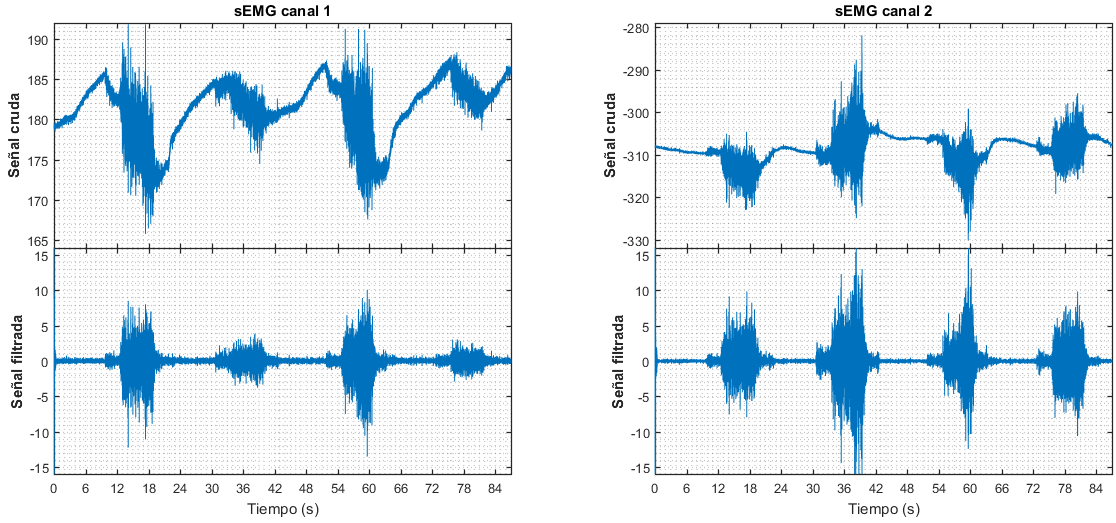
\includegraphics[width=\textwidth]{Filtrado.png}
	\caption{Ejemplo representativo del funcionamiento de los filtros diseñados aplicados a registros de entrenamiento.}
	\label{Figura: Filtrado}
\end{figure}

Con los registros ya filtrados se obtuvo el valor RMS a lo largo de todo el registro utilizando ventanas de 100 ms, dando como resultado una envolvente discreta de sEMG para cada canal. En la Figura \ref{Figura: RMS} se muestran los registros de sEMG filtrados con sus respectivas envolventes discretas de RMS y marcadores de la acción solicitada al sujeto durante el entrenamiento.

\begin{figure}[htbp]
	\centering
	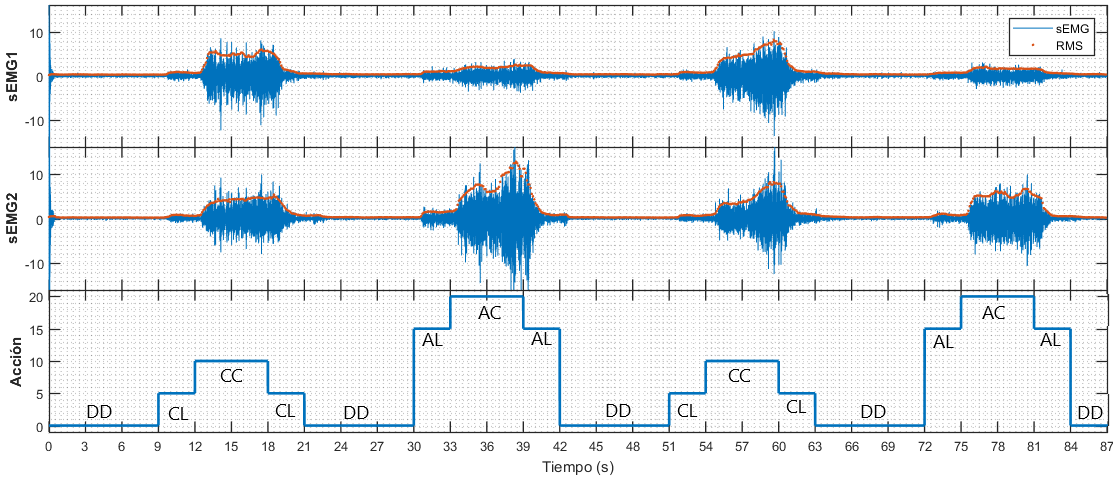
\includegraphics[width=\textwidth]{RMS_m.png}
	\caption{Ejemplo representativo de la obtención de envolvente discreta de RMS en registros de entrenamiento. Arriba: Canal 1 de sEMG. Medio: Canal 2 de sEMG. Abajo: Marcadores de acción solicitada al sujeto (descanso (DD), cierre ligero (CL), cierre completo (CC), apertura ligera (AL), apertura completa (AC)). Las envolventes (puntos rojoss) fueron multiplicadas por 2 para fines de visualización.}
	\label{Figura: RMS}
\end{figure}

\section{Esquema de control}
Previo a realizar pruebas del esquema de control en línea, este se probó fuera de línea, aprovechando los registros de calibración. Para estas pruebas se diseñó un script en MATLAB que obtiene los parámetros necesarios del esquema de control de la misma forma que los arroja la calibración. Una vez obtenidos dichos parámetros se configura con ellos al esquema de control y se realiza una prueba fuera de línea donde con cada ventana de sEMG se obtiene un valor de RMS el cuál es sometido al esquema de control y arroja un valor de amplitud para el canal asociado al movimiento detectado. Tras probar el esquema de control con tres registros distintos de calibración se obtuvo un porcentaje de acierto del 81$\%$ en la identificación correcta de los movimientos de cierre, apertura y descanso de mano.

En la Figura \ref{Figura: MapOff} se muestra el resultado de  una prueba exitosa del esquema de control fuera de línea, donde se observa que el esquema de control diseñado suele presentar errores en la identificación de los segmentos iniciales y finales de la tarea apertura de mano.

\begin{figure}[htbp]
	\centering
	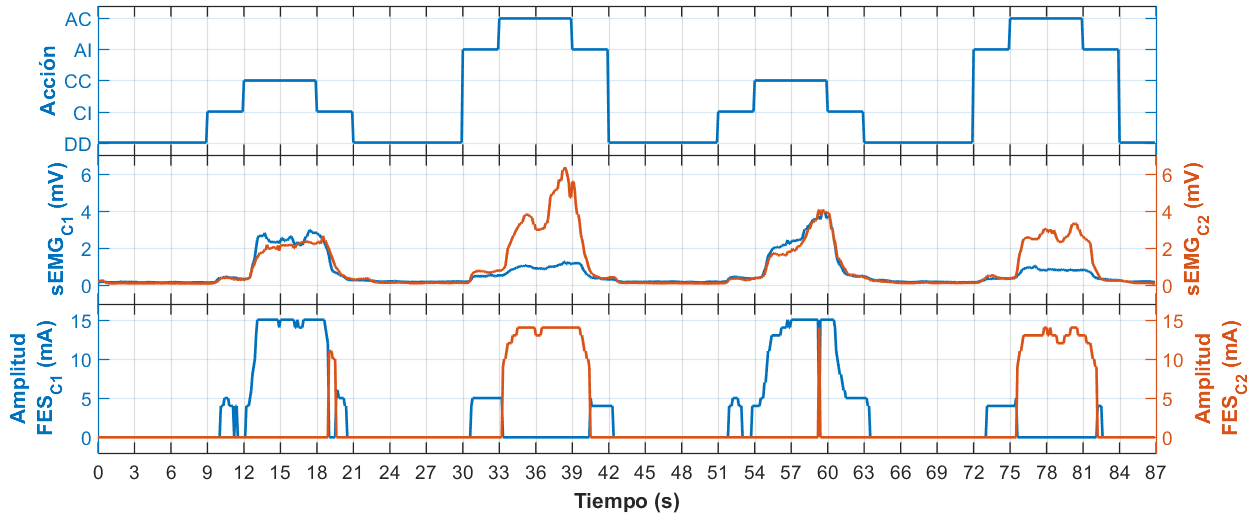
\includegraphics[width=\textwidth]{MapOff.png}
	\caption{Ejemplo exitoso representativo de las pruebas del sistema de control fuera de línea utilizando registros de entrenamiento. Arriba: Envolventes de sEMG (Azul: canal 1. Rojo: canal 2). Medio: Amplitudes de estimulación resultantes del sistema de control (Azul: canal 1. Rojo: canal 2). Abajo: Marcadores de acción solicitada al sujeto (descanso (DD), cierre ligero (CL), cierre completo (CC), apertura ligera (AL), apertura completa (AC)).}
	\label{Figura: MapOff}
\end{figure}



